\newcommand{\chapter}[2][]{
	\newcommand{\chapname}{#2}
	\begin{flushleft}
		\begin{minipage}[t]{\linewidth}
			
\includegraphics[height=1cm]{hdht-logo.png}
			\hspace{0pt}	
			\sffamily\bfseries\large Bài  1 + Bài 2 + Bài 3.
			\begin{flushleft}
				\LARGE\bfseries #1
			\end{flushleft}
		\end{minipage}
	\end{flushleft}
	\vspace{1cm}
	\normalfont\normalsize
}
\chapter[Làm quen với vật lí \\ Phương pháp nghiên cứu vật lí \\ Sai số khi đo các đại lượng vật lí \\ Các quy tắc an toàn trong phòng thực hành vật lí]{Làm quen với vật lí - Phương pháp nghiên cứu vật lí \\ Sai số khi đo các đại lượng vật lí \\Các quy tắc an toàn trong phòng thực hành vật lí}
\section{Lý thuyết}
%\subsection{Các đơn vị thường dùng trong vật lí học}
%\subsubsection{Đơn vị cơ bản}
%\begin{longtable}{|c|m{11em}|m{13em}|m{8em}|}
%	\hline
%	\thead{TT} & \thead{Đại lượng} & \thead{Tên đơn vị} & \thead{Kí hiệu đơn vị}
%	\\
%	\hline	
%	1 & Độ dài & mét & m 
%	\\
%	\hline	
%	2 & Khối lượng & kilôgam & kg
%	\\
%	\hline	
%	3 & Thời gian & giây & s
%	\\
%	\hline	
%	4 & Cường độ dòng điện & ampe & A 
%	\\
%	\hline	
%	5 & Nhiệt độ & kenvin & K
%	\\
%	\hline	
%	6 & Lượng chất & mol & mol
%	\\
%	\hline	
%	7 & Cường độ sáng & candela & cd
%	\\
%	\hline	

%\end{longtable}
%\subsubsection{Đơn vị dẫn xuất}
%\begin{longtable}{|c|m{11em}|m{13em}|m{8em}|}
%	\hline
%	\thead{TT} & \thead{Đại lượng} & \thead{Tên đơn vị} & \thead{Kí hiệu đơn vị}
%	\\
%	\hline	
%	\multicolumn{4}{|c|}{\textbf{Đơn vị không gian, thời gian và hiện tượng tuần hoàn}}
%	\\
%	\hline	
%	1 & Góc phẳng & rađian & rad 
%	\\
%	\hline	
%	2 & Diện tích & mét vuông & m$^2$
%	\\
%	\hline	
%	3 & Thể tích & mét khối & m$^3$
%	\\
%	\hline	
%	4 & Tần số & héc & Hz 
%	\\
%	\hline	
%	5 & Vận tốc góc & rađian trên giây & rad/s
%	\\
%	\hline	
%	6 & Gia tốc góc & rađian trên giây bình phương & rad/s$^2$
%	\\
%	\hline	
%	7 & Vận tốc & mét trên giây & m/s
%	\\
%	\hline	
%	8 & Gia tốc & mét trên giây bình phương & m/s$^2$
%	\\
%	\hline	
%		\multicolumn{4}{|c|}{\textbf{Đơn vị cơ}}
%	\\
%	\hline	
%	9 & Khối lượng riêng & kilôgam trên mét khối & kg/m$^3$ 
%	\\
%	\hline	
%	10 & Lực & niutơn & N
%	\\
%	\hline	
%	11 & Moment lực & niutơn mét & \SI{}{\newton.\meter}
%	\\
%	\hline	
%	12 & Áp suất & pascan & Pa 
%	\\
%	\hline	

%\end{longtable}

\subsection{Đối tượng nghiên cứu của vật lí và mục tiêu của môn vật lí}
\subsubsection{Đối tượng nghiên cứu của vật lí}
Vật lí là môn ``khoa học tự nhiên'' có đối tượng nghiên cứu tập trung vào các dạng vận động của vật chất (chất, trường), năng lượng.
\subsubsection{Mục tiêu học tập môn vật lí}
Giúp các em hình thành, phát triển năng lực vật lí:
\begin{itemize}
	\item Có được những kiến thức, kĩ năng cơ bản về vật lí.
	\item Vận dụng được kiến thức, kĩ năng đã học để khám phá, giải quyết các vấn đề có liên quan trong học tập cũng như trong đời sống.
	\item Nhận biết được năng lực, sở trường của bản thân, định hướng nghề nghiệp.
\end{itemize}
\subsection{Quá trình phát triển của vật lí}
\begin{center}
	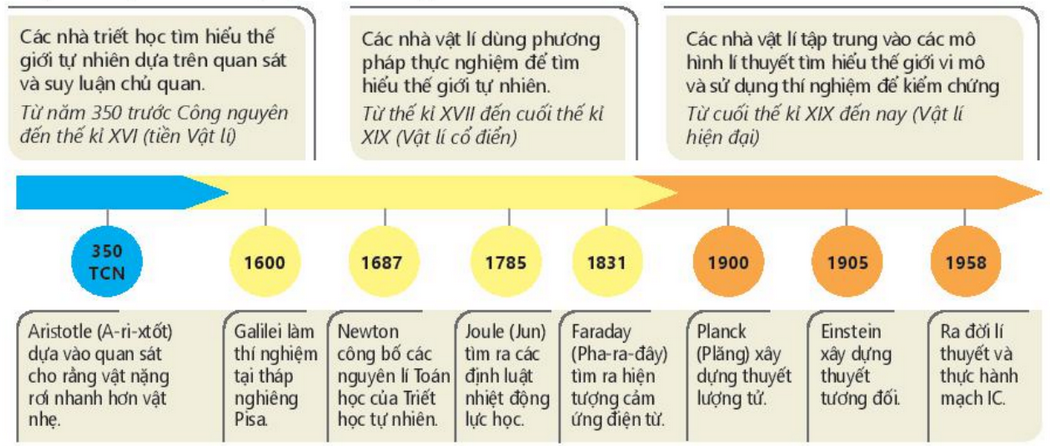
\includegraphics[width=0.95\textwidth]{../figs/G10-1-1}
\end{center}

\subsection{Vai trò của vật lí đối với khoa học, kĩ thuật và công nghệ}
	\begin{description}
		\item[Đối với khoa học:] Vật lí được coi là cơ sở của khoa học tự nhiên. Các khái niệm, định luật, nguyên lý của Vật lí được áp dụng trong tất cả lĩnh vực khoa học tự nhiên. 
		\item[Đối với kỹ thuật và công nghệ:] Vật lí là cơ sở của công nghệ và các ngành kỹ thuật. Có thể khẳng định: không có thành tựu của Vật lí thì không có công nghệ.  
	\end{description}
%\begin{center}
%	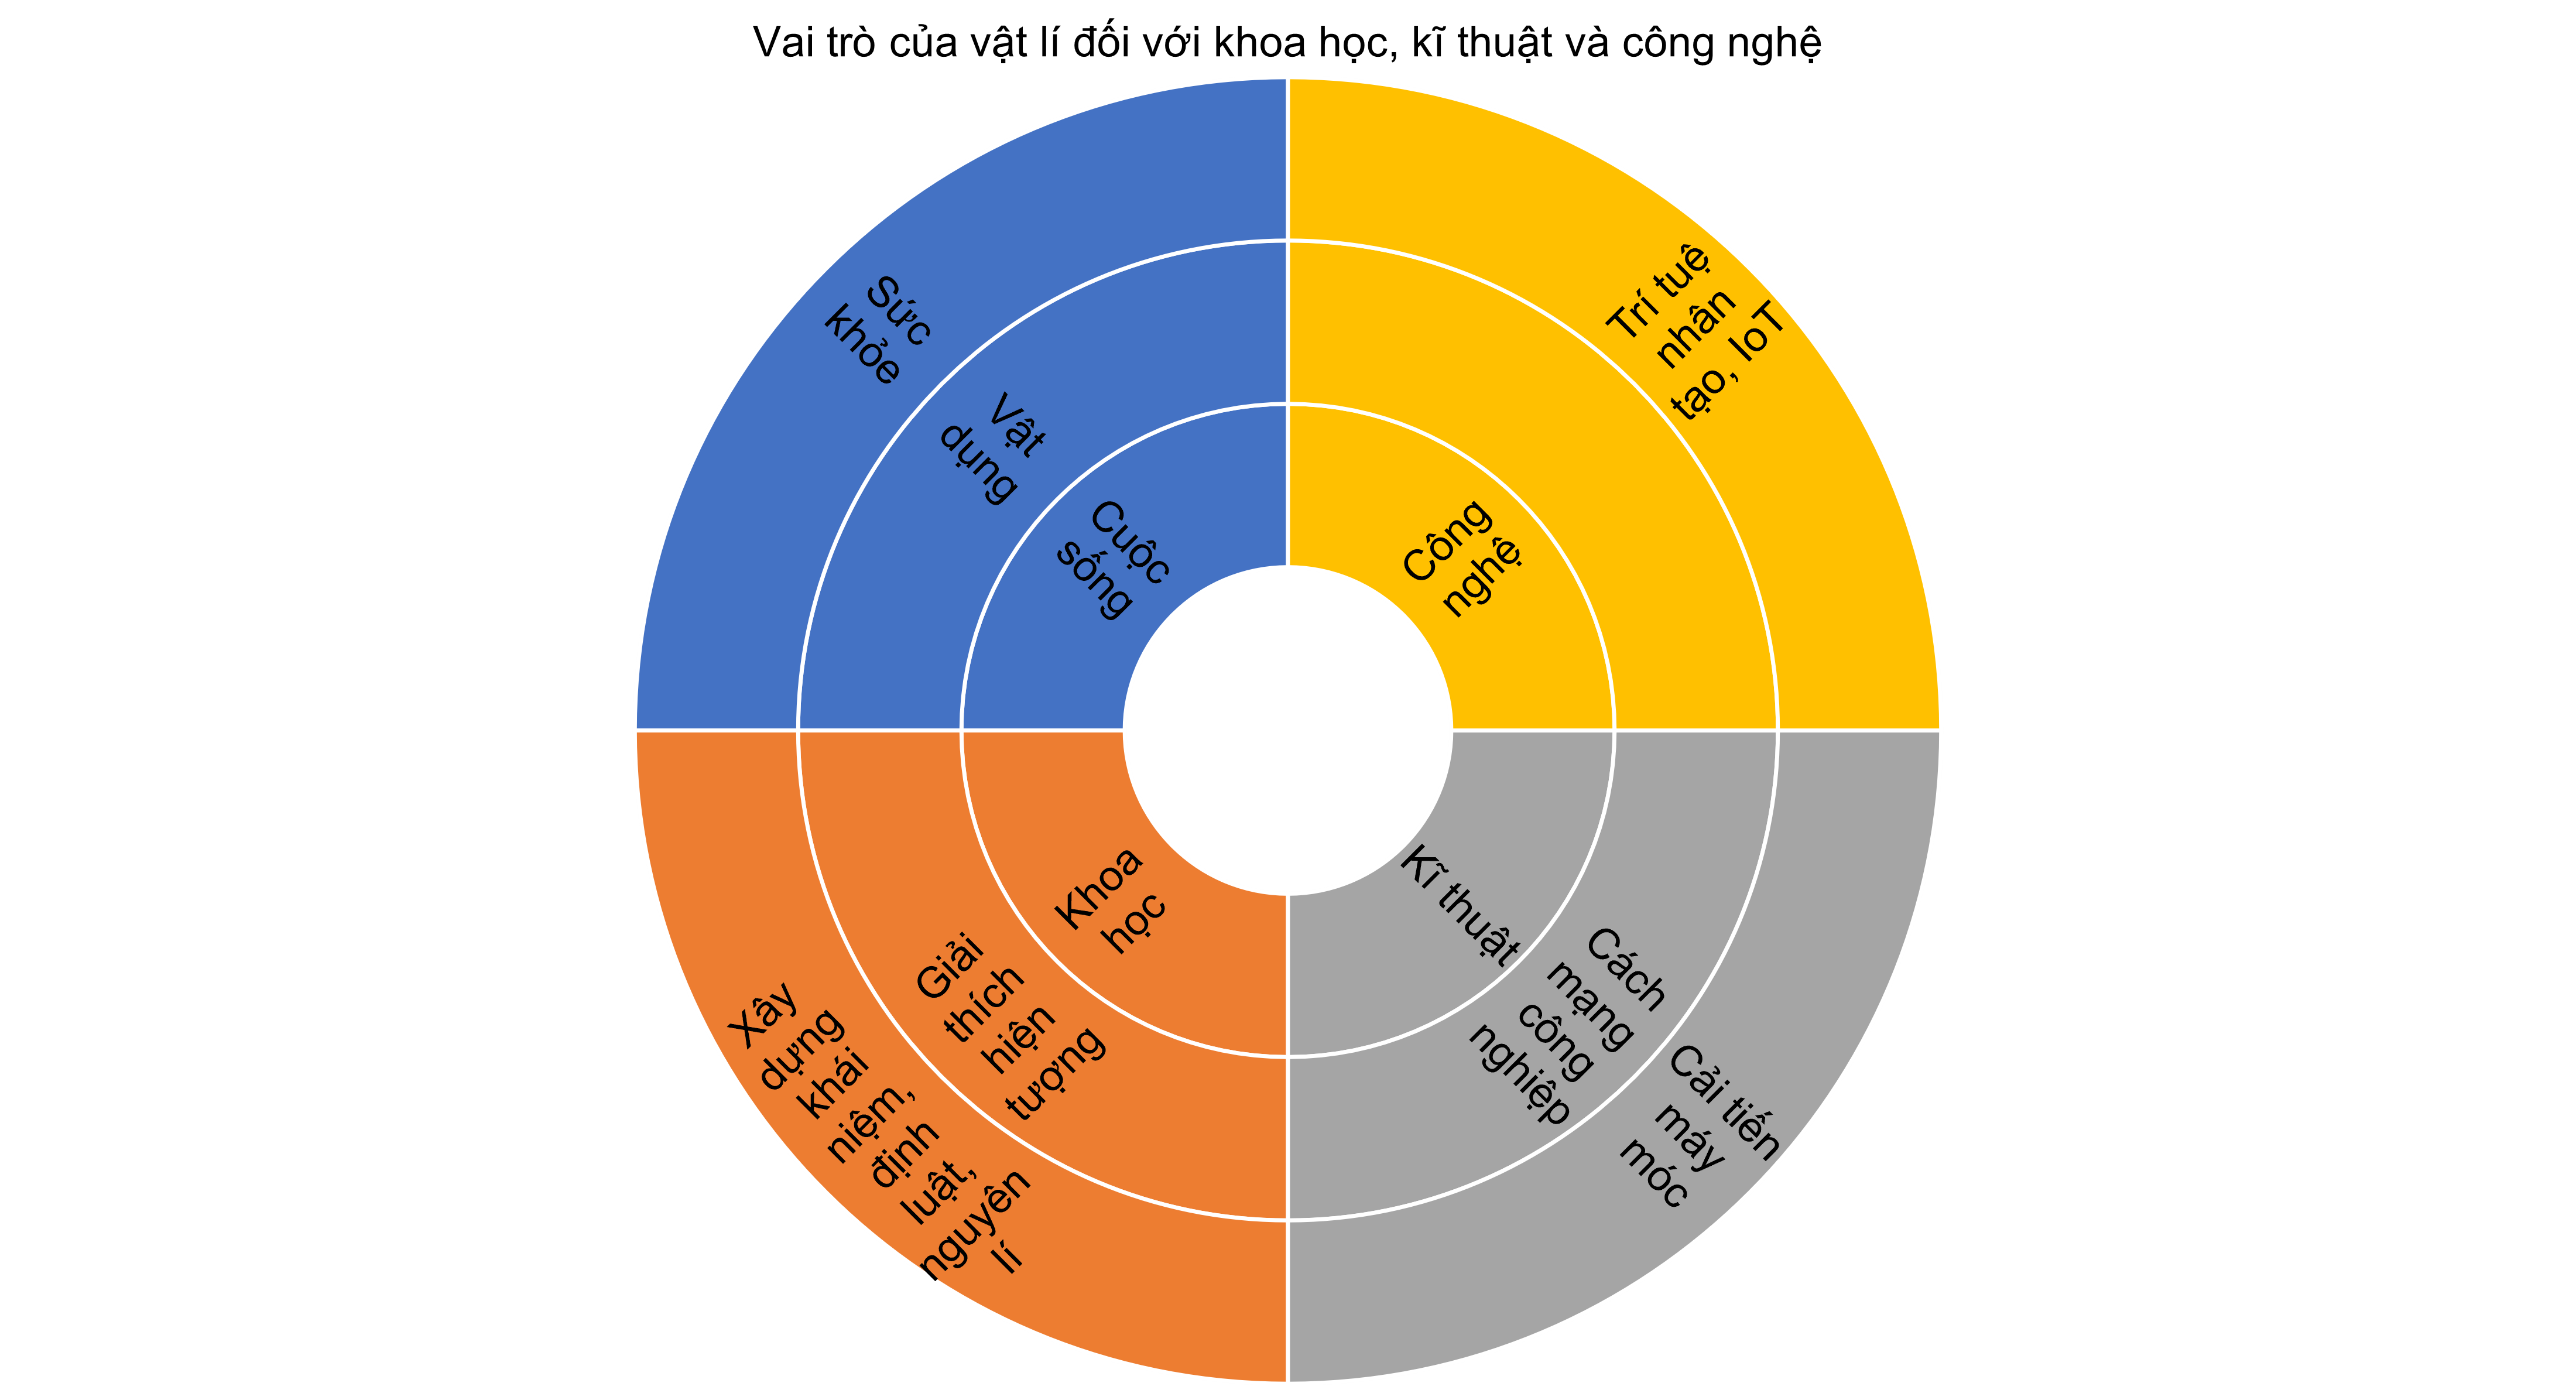
\includegraphics[scale=0.4]{../figs/G10-1-3}
%\end{center}
\subsection{Phương pháp nghiên cứu vật lí}
\subsubsection{Phương pháp thực nghiệm}
\begin{center}
	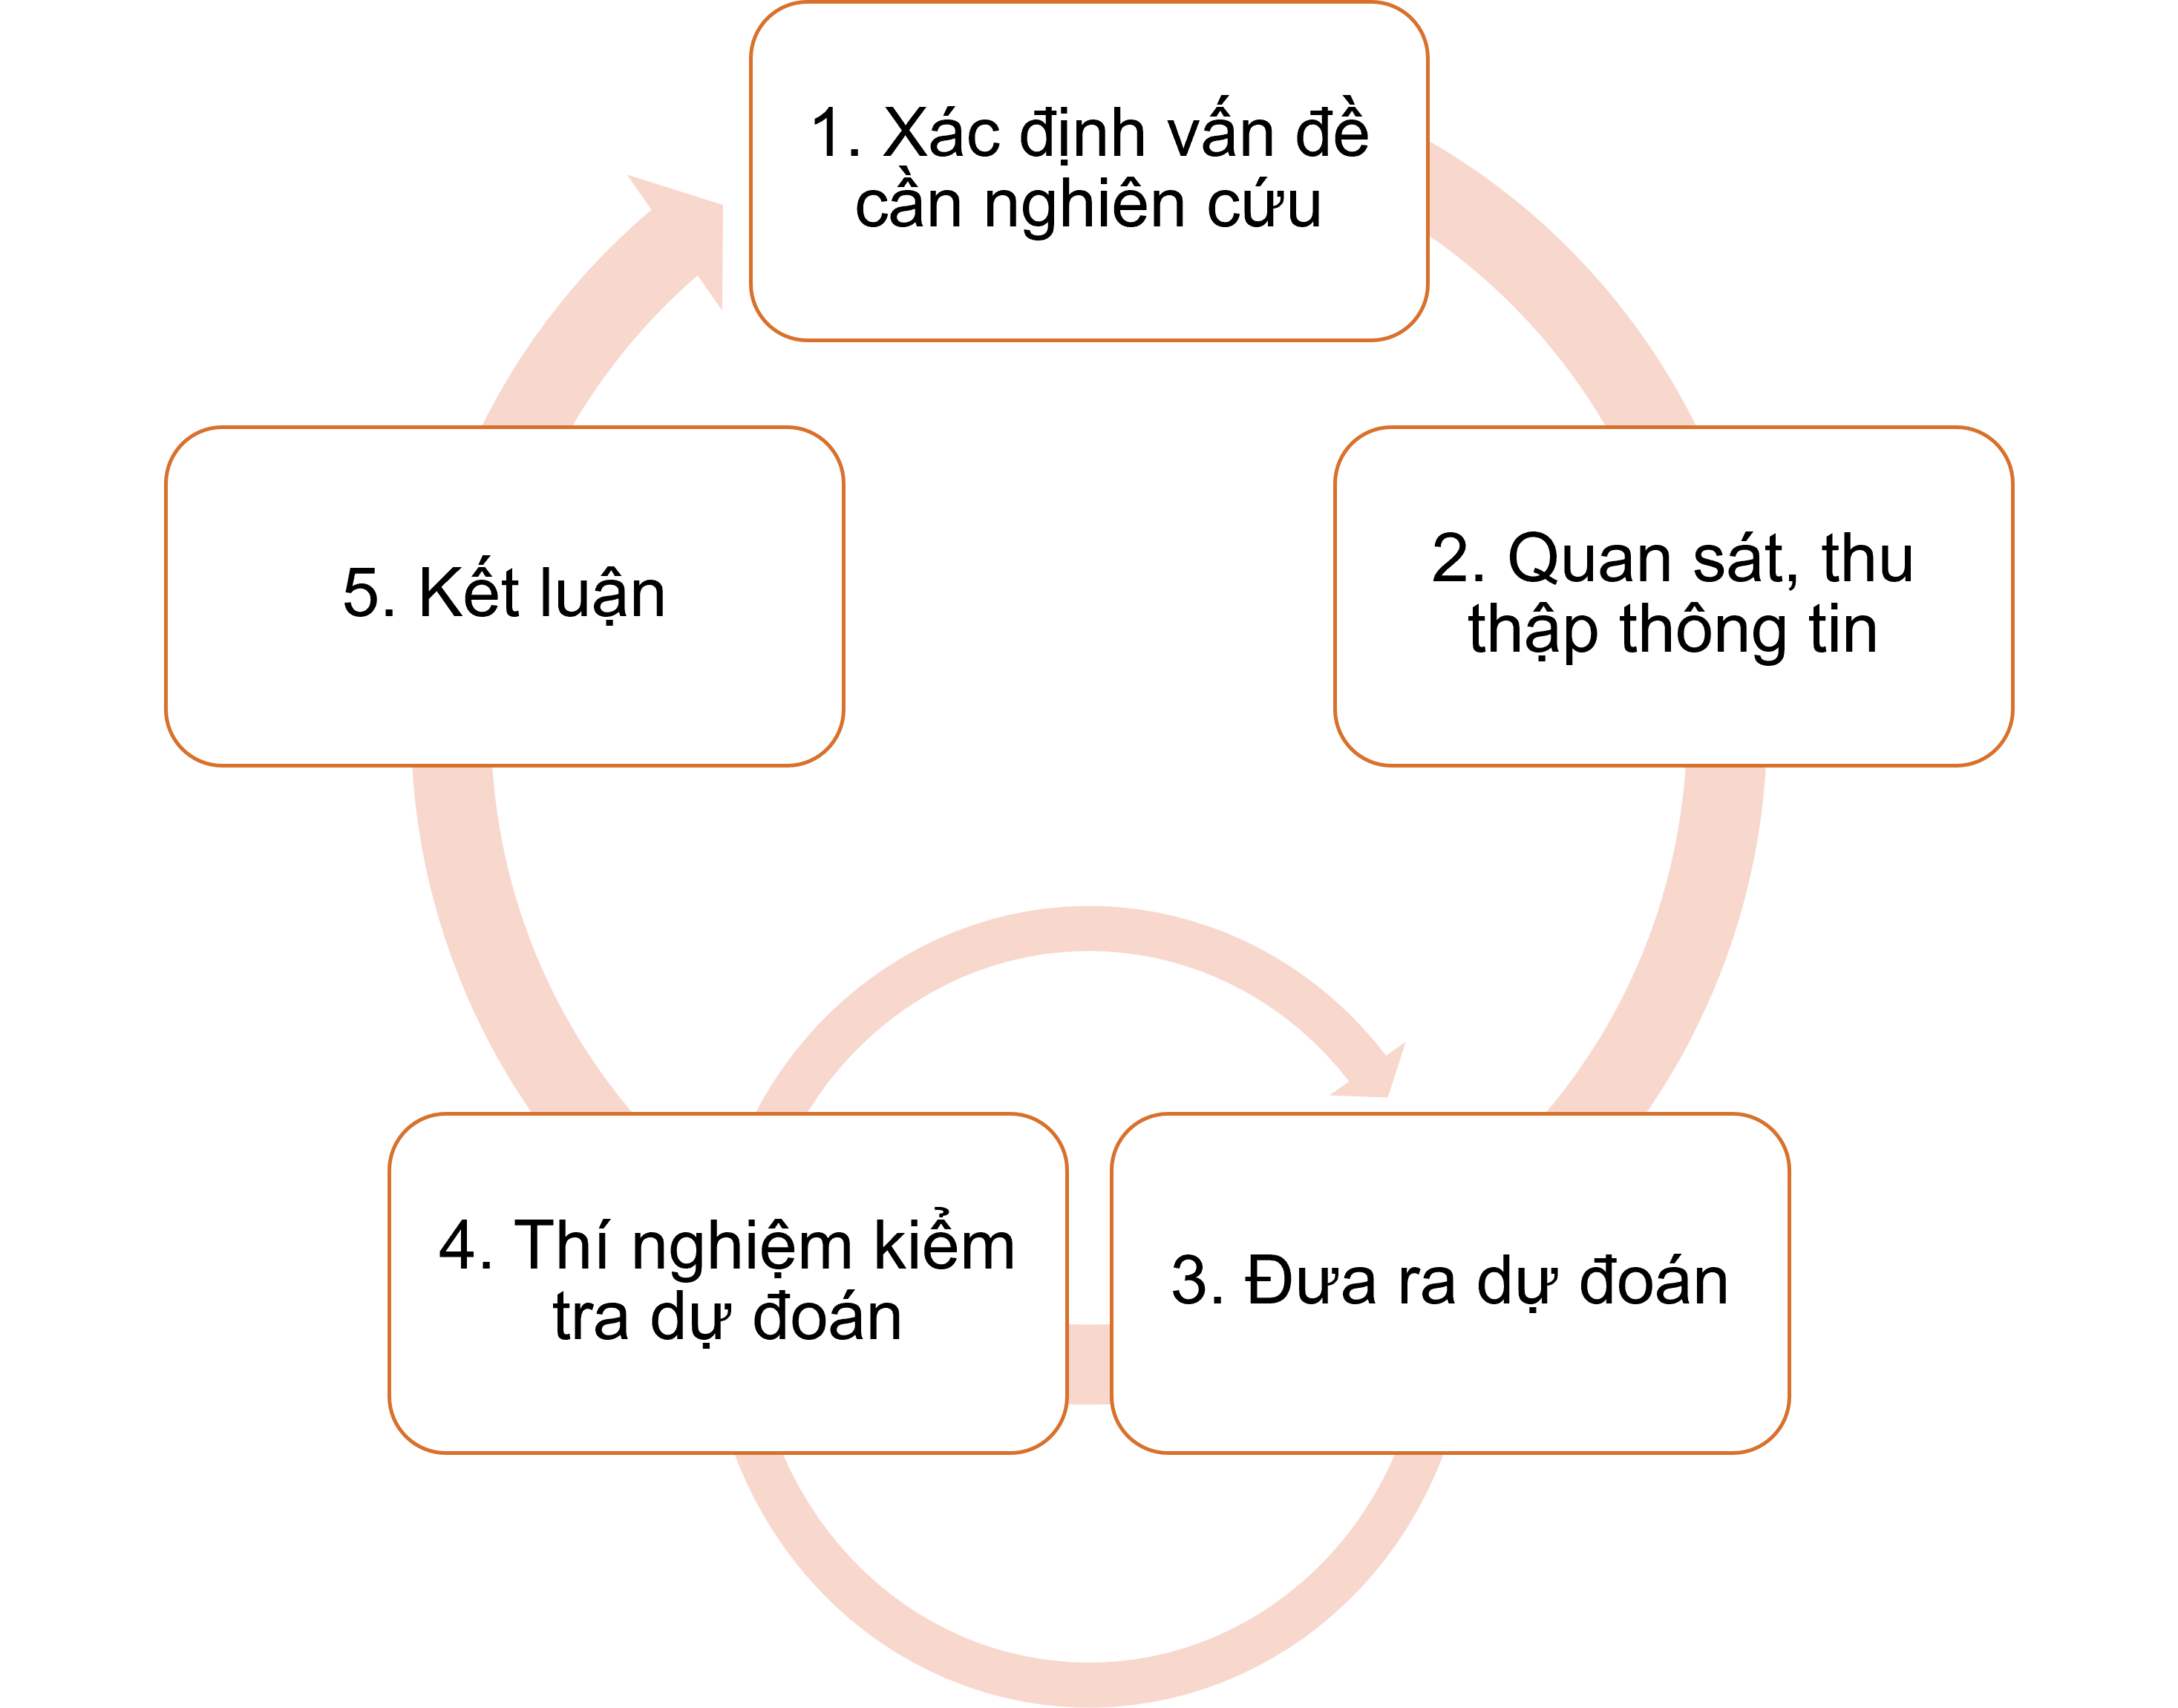
\includegraphics[scale=0.4]{../figs/G10-1-2}
\end{center}
\subsubsection{Phương pháp mô hình}
\begin{center}
	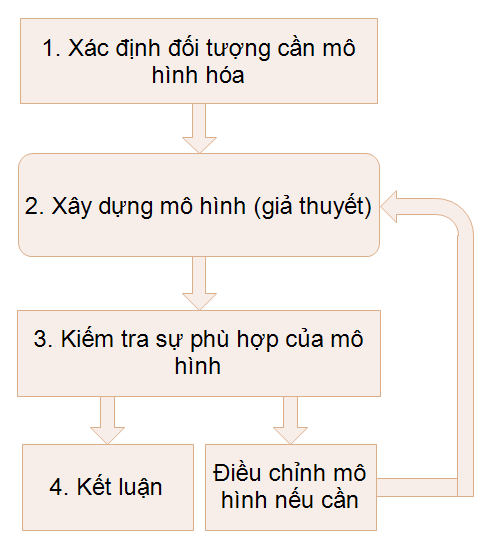
\includegraphics[scale=0.7]{../figs/G10-1-4}
\end{center}
	\subsection{Phép đo các đại lượng vật lí - Hệ SI}
\subsubsection{Phép đo các đại lượng vật lí}
Phép đo một đại lượng vật lí là phép so sánh nó với đại lượng cùng loại được quy ước làm đơn vị.

Phép đo được phân loại thành 
	\begin{itemize}
		\item \textbf{Phép đo trực tiếp} là phép xác định giá trị  một đại lượng bằng cách so sánh trực tiếp với dụng cụ đo. 
		\item \textbf{Phép đo gián tiếp} là phép xác định giá trị một đại lượng thông qua một công thức liên hệ với các đại lượng được đo trực tiếp.   
	\end{itemize}
\subsubsection{Hệ đơn vị đo}
Một hệ thống các đơn vị đo các đại lượng vật lí được quy định thống nhất áp dụng tại nhiều nước trên thế giới, trong đó có Việt Nam.

Hệ đơn vị được sử dụng phổ biến trong đời sống là hệ SI, được xây dựng trên cơ sở của 7 đơn vị đo lường cơ bản như  trong bảng bên dưới. Các đơn vị này được sử dụng để định nghĩa các đơn vị đo lường khác.  
	\begin{longtable}{|c|m{11em}|c|c|}
			\hline
			\thead{TT} & \thead{Đại lượng} & \thead{Tên đơn vị} & \thead{Kí hiệu đơn vị}
			\\
			\hline	
			1 & Độ dài & mét & m 
			\\
			\hline	
			2 & Khối lượng & kilôgam & kg
			\\
			\hline	
			3 & Thời gian & giây & s
			\\
			\hline	
			4 & Cường độ dòng điện & ampe & A 
			\\
			\hline	
			5 & Nhiệt độ & kenvin & K
			\\
			\hline	
			6 & Lượng chất & mol & mol
			\\
			\hline	
			7 & Cường độ sáng & candela & cd
			\\
			\hline	
	\end{longtable}	
\subsection{Giá trị trung bình}
Khi đo $n$ lần cùng một đại lượng $A$, ta thu được các giá trị khác nhau: $A_1,\, A_2,\,...,A_n$

Giá trị trung bình khi đo nhiều lần một đại lượng $A$:$$\bar{A}=\dfrac{A_1+A_2+...+A_{\text{n}}}{n},$$
là giá trị gần đúng nhất với giá trị thực của đại lượng $A$.  
\subsection{Sai số phép đo}
\subsubsection{Phân loại sai số}
Sai số phép đo bao gồm \bltext{sai số dụng cụ} và \bltext{sai số ngẫu nhiên}.

\subsubsection{Cách xác định sai số của phép đo trực tiếp}
\begin{itemize}
	\item Sai số tuyệt đối ứng với mỗi lần đo:
	$$\Delta A_1=|\bar{A}-A_1|;\,\Delta A_2=|\bar{A}-A_2|;\,\Delta A_3=|\bar{A}-A_3|;...$$
	\item Sai số ngẫu nhiên là sai số tuyệt đối trung bình của $n$ lần đo:
	$$\overline{\Delta A}=\dfrac{\Delta A_1+\Delta A_2+...+\Delta A_{\textrm{n}} }{n}.$$
	\item Sai số dụng cụ $\Delta A'$ có thể lấy bằng nửa hoặc một độ chia nhỏ nhất trên dụng cụ.
	\item Sai số tuyệt đối của phép đo là tổng \bltext{sai số ngẫu nhiên} và \bltext{sai số dụng cụ}:
	$$\Delta A= \overline{\Delta A}+ \Delta A'.$$
\end{itemize}
\subsubsection{Sai số tỉ đối}
Sai số tỉ đối $\delta A$ của phép đo là tỉ số giữa \bltext{sai số tuyệt đối} và \bltext{giá trị trung bình} của đại lượng cần đo, tính bằng phần trăm:
$$\delta A=\dfrac{\Delta A}{\overline A}\cdot 100\%.$$
Sai số tỉ đối càng \bltext{nhỏ} thì phép đo càng chính xác.

\subsubsection{Cách xác định sai số của phép đo gián tiếp}
Sai số của phép đo gián tiếp, được xác định theo các quy tắc:
\begin{itemize}
\item Sai số tuyệt đối của một tổng hay hiệu thì bằng \bltext{tổng} các sai số tuyệt đối của các số hạng.
\item Sai số tỉ đối của một tích hay thương thì bằng \bltext{tổng} các sai số tỉ đối của các thừa số. 
\end{itemize}
\subsection{Cách viết kết quả đo}
$$A=\overline{A} \pm \Delta A,$$
trong đó:
\begin{itemize}
	\item $\overline A$ là giá trị trung bình,
	\item $\Delta A$ là sai số tuyệt đối. 
\end{itemize}

\subsection{Một số quy định về an toàn trong phòng thực hành vật lí}
\subsubsection{Quy tắc an toàn trong sử dụng các thiết bị điện}
Cần quan sát kĩ các kí hiệu và nhãn thông số trên thiết bị để sử dụng đúng chức năng, đúng yêu cầu kĩ thuật.

Một số kí hiệu trên các thiết bị thí nghiệm:
\begin{center}
	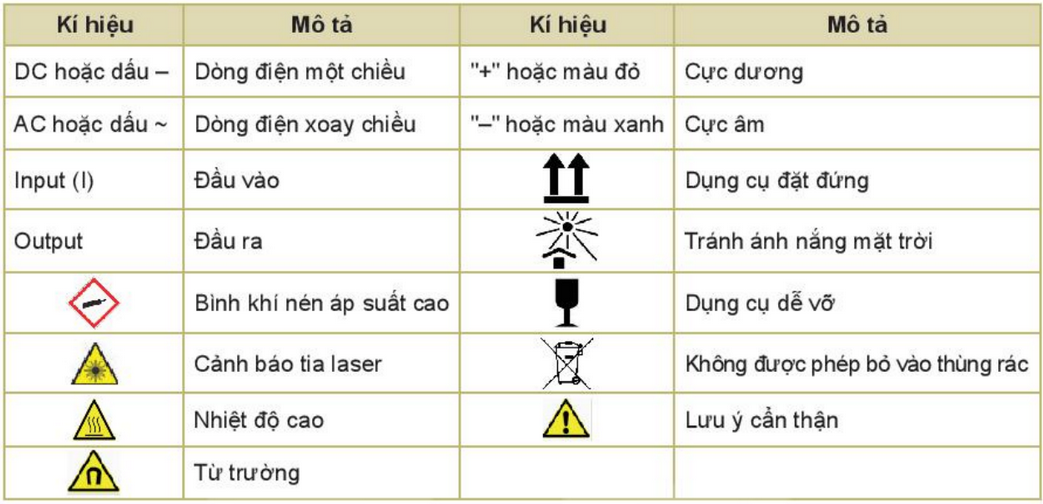
\includegraphics[scale=0.7]{../figs/G10-2-1}
\end{center}
\subsubsection{Quy tắc an toàn sử dụng các thiết bị nhiệt và thủy tinh}
Các thiết bị đun nóng có thể gây cháy hoặc nứt, vỡ các dụng cụ bằng thuỷ tinh.
\subsubsection{Quy tắc an toàn sử dụng các thiết bị quang học}
Các thiết bị quang học rất dễ bị mốc, xước, nứt, vỡ và dính bụi bẩn, làm ảnh hưởng đến đường truyền tia sáng và sai lệch kết quả thí nghiệm.
\section{Mục tiêu bài học - Ví dụ minh họa}
\begin{dang}{Nêu được đối tượng nghiên cứu của\\ vật lí học và mục tiêu của môn Vật lí}
	\viduii{1}{Hãy kể tên các lĩnh vực vật lí mà em đã được học ở cấp Trung học cơ sở.
	}
	{	\begin{center}
			\textbf{Hướng dẫn giải}
		\end{center}
		
	Ở cấp Trung học cơ sở, vật lí nghiên cứu các vấn đề cơ bản nhất của vật lí học, có thể kể đến như:
	\begin{itemize}
%		\item Đo lường và các dụng cụ đo lường;
		\item Cơ học: Các chuyển động cơ học đơn giản, chuyển động dưới tác dụng của lực, năng lượng cơ học (cơ năng);
		\item Nhiệt học: Các đại lượng đặc trưng trong nhiệt học;
		\item Âm học: Các hiện tượng liên quan đến âm thanh;
		\item Điện học: Các mạch điện chứa điện trở, định luật cơ bản trong điện học;
		\item Quang học: Các dụng cụ quang học thường gặp, các định luật quang hình học.
	\end{itemize}
	}
	\viduii{1}{Học tốt môn vật lí sẽ giúp ích gì cho em?
	}
	{	\begin{center}
			\textbf{Hướng dẫn giải}
		\end{center}
	
		Em hãy trao đổi với giáo viên và bày tỏ suy nghĩ của mình.
	}
\end{dang}

\begin{dang}{Phân tích được một số ảnh hưởng của vật lí đối với cuộc sống, đối với sự phát triển \\của khoa học, công nghệ và kĩ thuật}
	\viduii{1}{Lấy ví dụ chứng tỏ tri thức vật lí giúp tránh được nguy cơ tổn hại về sức khỏe.
	}
	{	\begin{center}
			\textbf{Hướng dẫn giải}
		\end{center}
		
		Các em có thể lấy ví dụ vào các lĩnh vực nằm trong hiểu biết của mình:
		\begin{itemize}
			\item Kỹ thuật: chế tạo các công cụ, máy móc giúp tiết kiệm sức lao động;
			\item Công nghệ: chế tạo robot để thực hiện những công việc nguy hiểm;
			\item Y sinh: phẫu thuật Laser, nội soi, làm đẹp và thẫm mỹ, $\ldots$; 
			\item Y học dự phòng: thói quen sinh hoạt, làm việc khoa học dựa trên hoạt động của cơ, xương khớp;
			\item Vật lí trị liệu: kích hoạt huyệt đạo trên cơ thể bằng dòng điện, châm cứu, hồng ngoại, tử ngoại, $\ldots$.
		\end{itemize}
	}
	\viduii{1}{Lấy ví dụ và phân tích ảnh hưởng của vật lí đối với sự phát triển của khoa học kĩ thuật và công nghệ
	}
	{\begin{center}
			\textbf{Hướng dẫn giải}
		\end{center}
		
		Các em có thể lấy ví dụ vào các lĩnh vực nằm trong hiểu biết của mình:
		\begin{itemize}
			\item Công nghiệp: máy móc công nghiệp hoạt động dựa trên các nguyên lí về dòng điện và từ trường;
			\item Nông nghiệp: hệ thống chăm sóc nông nghiệp tự động hóa dựa trên các nghiên cứu lượng tử.
			\item Dịch vụ: y tế, đời sống xã hội, giao thông, $\ldots$.
		\end{itemize}
	}
\end{dang}

\begin{dang}{Nêu được ví dụ về \\ các phương pháp nghiên cứu vật lí \\(thực nghiệm và lí thuyết)}
	\viduii{1}
	{Lấy ví dụ về một kiến thức được hình thành từ quan sát thực nghiệm}
	{\begin{center}
			\textbf{Hướng dẫn giải}
	\end{center}
	
	Những vấn đề thường được kể đến là
	\begin{itemize}
		\item Sự rơi của một vật;
%		\item Chuyển động của một vật khi không có ma sát;
		\item Chuyển động của Trái Đất quay quanh Mặt Trời; 
		\item Sự nổi của một vật.
		\item Nguyên lý của đòn bẩy.
	\end{itemize}
	}
\end{dang}
\begin{dang}{Mô tả được các bước \\trong tiến trình tìm hiểu thế giới tự nhiên}
	\viduii{1}
	{Hãy kể tên một số mô hình thí nghiệm mà em thấy trong phòng thí nghiệm Vật lí ở trường phổ thông.}
	{\begin{center}
			\textbf{Hướng dẫn giải}
	\end{center}
	
	Những mô hình thường có trong phòng thí nghiệm Vật lí ở trường phổ thông là
	\begin{itemize}
		\item Mô hình khảo sát sự rơi của vật nặng;
		\item Mô hình khảo sát chuyển động thẳng đều trên đệm không khí;
		\item Mô hình con lắc, dây đàn hồi có sóng dừng.
		\item Mô hình khảo sát lực căng bề mặt của chất lỏng.
		\item \ldots
	\end{itemize}
	}
\end{dang}
\begin{dang}{Xác định được sai số tuyệt đối,\\ sai số tỉ đối và biểu diễn được kết quả đo}
	\viduii{3}{Trong bài thực hành đo gia tốc trọng trường của Trái Đất tại phòng thí nghiệm, một học sinh đo được chiều dài của con lắc đơn $l= \SI{800(1)}{\milli\meter}$ thì chu kì dao động là $T = \SI{1.78(0.02)}{\second}$. Lấy $\pi=\SI{3.14}{}$. Biết chu kỳ của con lắc đơn tính theo công thức $T=2\pi \sqrt{l/g}$. Gia tốc trọng trường $g$ của Trái Đất tại phòng thí nghiệm đó là bao nhiêu?
	}
	{	\begin{center}
			\textbf{Hướng dẫn giải}
		\end{center}
		
		Từ công thức: $$T=2\pi \sqrt{\dfrac{l}{g}} \Rightarrow g=\dfrac{4\pi^2l}{T^2}.$$ 	
		
		Giá trị trung bình của gia tốc trọng trường: 	
		$$\overline{g}=\dfrac{4\pi^2l}{T^2}=\dfrac{4\pi^2\cdot \SI{3.14}{}^2\cdot \SI{0.8}{\meter}}{\left( \SI{1.78}{\second}\right)^2}=\SI{9.96}{\meter\per\second^2}.$$
		
		Sai số tuyệt đối của gia tốc trọng trường:
			\begin{align*}
				\dfrac{\Delta g}{\overline g}&= \dfrac{\Delta l}{\overline l}+ 2\dfrac{\Delta T}{\overline T}\\
				&=\dfrac{\SI{1}{\milli\meter}}{\SI{800}{\milli\meter}}+2\times\dfrac{\SI{0.02}{\second}}{\SI{1.78}{\second}}\\
				&=\SI{0.024}{}\\
				\Rightarrow\quad \Delta g&= \SI{0.024}{}\cdot \overline g\\
				&= \SI{0.24}{\meter\per\second^2}.
			\end{align*}
	
		
		
		Vậy gia tốc trọng trường của Trái Đất tại phòng thí nghiệm đó là
		$$g={\overline g } \pm \Delta g =\SI{9.96(0.24)}{\meter\per\second^2}.$$
	}
	\viduii{3}{Một học sinh dùng cân và đồng hồ đếm giây để đo độ cứng $k$ của lò xo. Dùng cân để cân vật nặng thu được kết quả khối lượng $m = 100 \,\text{g}$ với sai số tỉ đối là $2\%$. Gắn vật vào lò xo và kích thích cho con lắc dao động rồi dùng đồng hồ đếm giây đo thời gian của một dao động cho kết quả $T = 2\,\text{s}$ với sai số tỉ đối là $1\%$. Biết chu kỳ của con lắc lò xo tính theo công thức $T=2\pi \sqrt{m/k}$. Sai số tỉ đối của phép đo độ cứng của lò xo là bao nhiêu?
	}
	{	\begin{center}
			\textbf{Hướng dẫn giải}
		\end{center}
		
		Từ công thức: $$T=2\pi \sqrt{\dfrac{m}{k}} \Rightarrow k=\dfrac{4\pi^2m}{T^2}.$$	
		
		Sai số tỉ đối của độ cứng lò xo: 	
		$$\dfrac{\Delta k}{\overline k}= \dfrac{\Delta m}{\overline m}+ 2\dfrac{\Delta T}{\overline T}= 2\%+2\cdot 1\%= 4\%.$$
		
		Vậy sai số tỉ đối của phép đo độ cứng của lò xo là $4\%.$
	}
\end{dang}

\begin{dang}{Vận dụng được các quy tắc an toàn \\trong phòng thực hành vật lí}
	\viduii{2}{Hãy nêu quy tắc an toàn trong việc sử dụng các thiết bị sau:
		\begin{enumerate}
			\item Phích cắm điện;
			\item Dây điện;
			\item Nguồn tia LASER;
			\item Đèn cồn.
		\end{enumerate}
	}
	{	\begin{center}
			\textbf{Hướng dẫn giải}
		\end{center}
		
		\begin{enumerate}
			\item Phích cắm điện: Không chạm tay vào vị trí tiếp xúc giữa phích cắm và ổ điện, không cắm điện khi tay ướt.
			\item Dây điện: Không sử dụng dây điện cũ, không đấu nối dây điện thiếu an toàn.
			\item Nguồn tia LASER: Không đặt mắt trực tiếp trên đường truyền của tia LASER, không chiếu tia LASER vào người khác;
			\item Đèn cồn: Không bỏ đi nơi khác khi đang đun bằng đèn cồn, hơ lửa đều để ống nghiệm giãn nở đều.
		\end{enumerate}
	}
	\viduii{2}{Hãy cho biết các dụng cụ đo sau có chức năng gì và cách nối chúng vào mạch điện:
		\begin{enumerate}
			\item Ampe kế;
			\item Vôn kế;
			\item Đồng hồ đo điện đa năng.
		\end{enumerate}
	}
	{\begin{center}
			\textbf{Hướng dẫn giải}
		\end{center}
		
		\begin{enumerate}
			\item Ampe kế: Dùng để đo cường độ dòng điện, nối tiếp với đoạn mạch cần đo;
			\item Vôn kế: Dùng để đo hiệu điện thế, mắc song song với đoạn mạch cần đo;
			\item Đồng hồ đo điện đa năng: Dùng để đo hiệu điện thế, cường độ dòng điện và điện trở, cần vặn núm xoay vào thang đo phù hợp trước khi tiến hành đo.
		\end{enumerate}
	}
\end{dang}